\chapter{Dynamic Programming}

\section{Knuth Optimization}

    Knuth's optimization, also known as the Knuth-Yao Speedup, is a special case of dynamic programming on ranges, that can optimize the time complexity of solutions by a linear factor, from $O(n^3)$ for standard range DP to $O(n^2)$.

\subsection{Conditions}

    The Speedup is applied for transitions of the form:

    $$dp(i, j) = \min_{i \leq k < j} [ dp(i, k) + dp(k+1, j) + C(i, j) ].$$

    Similar to divide and conquer DP, let $opt(i, j)$ be the value of $k$ that minimizes the expression in the transition ($opt$ is referred to as the "optimal splitting point" further in this article). The optimization requires that the following holds:

    $$opt(i, j-1) \leq opt(i, j) \leq opt(i+1, j).$$

    We can show that it is true when the cost function 
    $C$ satisfies the following conditions for $a \leq b \leq c \leq d$:

    $C(b, c) \leq C(a, d)$;

    $C(a, c) + C(b, d) \leq C(a, d) + C(b, c)$ (the quadrangle inequality [QI]).

    A common cost function that satisfies the above condition is the \textbf{sum of the values in a subaray}.

    \kactlimport{knuth.cpp}

\section{Slope}

\subsection{Convex Hull Trick}

    If multiple transitions of the DP can be seen as 
    first degree polynomials (lines). CHT can be used to optimized it

    Some valid functions:

    $ax + b$
    
    $cx^2 + ax + b$ 
    (ignore $cx^2$ if c is independent)

    \kactlimport{cht-dynamic.cpp}

\subsection{Li-chao Tree}

    Works for any type of function that has the \textbf{transcending property}:

    Given two functions f(x),g(x) of that type, 
    if f(t) is greater than/smaller than g(t) for some x=t,
    then f(x) will be greater than/smaller than g(x) for x>t.
    In other words, once f(x) “win/lose” g(x), f(x) will continue to “win/lose” g(x).

    The most common one is the line function: $ ax + b $

\section{SOS DP}

    \textbf{Sum over Subsets DP (SOS DP)} computes how many elements there are for each mask
    which are a subset of this mask.

    This can be modified for other operations in which the subset contributes for the mask
    .
    \textit{Example:}

    \textbf{10}0\textbf{1} if a subset of \textbf{11}0\textbf{1};

    \textbf{00}0\textbf{1} if a subset of \textbf{11}0\textbf{1};
    
    \textbf{11}0\textbf{0} if a subset of \textbf{11}0\textbf{1};
    
    \textbf{11}0\textbf{1} if a subset of \textbf{11}0\textbf{1};

    \begin{center}
        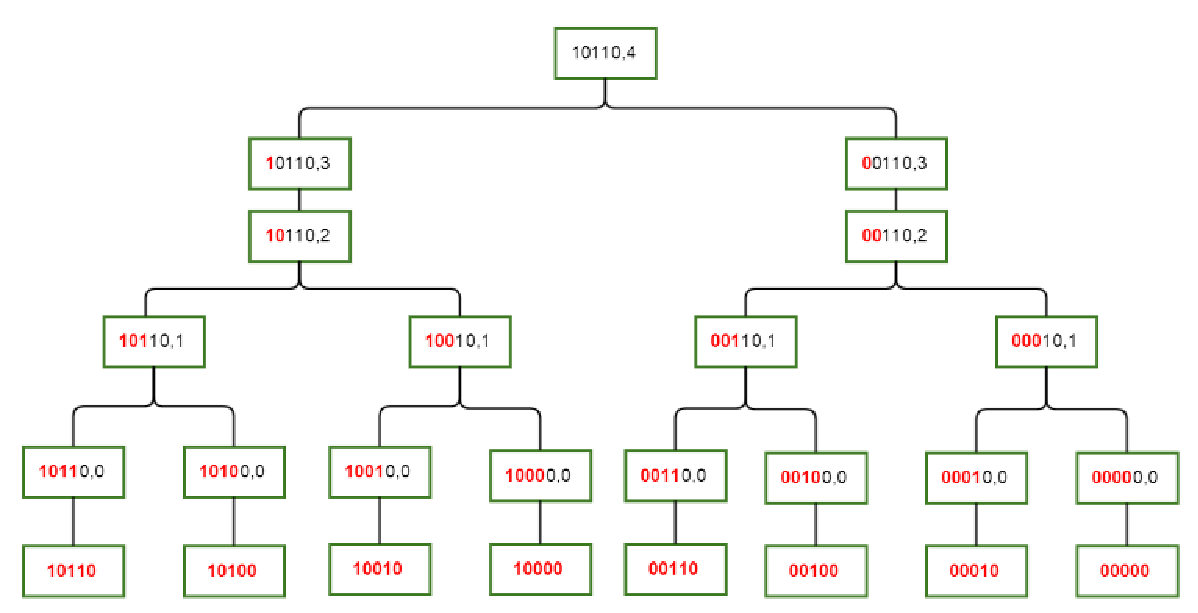
\includegraphics[width=9cm]{content/dynamic-programming/sos-example.pdf}
    \end{center}

    \kactlimport{sos-dp.cpp}